\section{Caracterización de la red actual}
\label{sec:caracterizacion}

La red considerada para el comienzo de este proyecto consiste en un
tendido de fibra óptica estándar tipo G.652.D\cite{G652D}. Cada enlace
de fibra óptica une un par de \emph{DC} de forma directa y sin
estaciones intermedias mediante cables de 96 fibras diseñadas para
operar en la banda C.

En un comienzo, cada fibra tiene soporte para un solo servicio usando
un par de transmisión y recepción Láser, filtros y amplificadores,
donde aplique. No se considerará ninguno de estos equipos
preexistentes en el diseño de fibra activa, salvo el tendido
preexistente.

Este tendido es de 399 Km distribuidos en 9 tramos con longitudes de
entre 10 y 132 Km. Tal y como está, el tendido no tiene considerado
ningún plan de contingencia que considere cortes de los cables, por lo
que no existen garantías de \emph{SLA} que establezcan políticas
claras de \emph{uptime} o \emph{delay} en el servicio (de haberlas,
estas se violarían sistemáticamente, causándole a la empresa
multas). Por otro lado, dado que las distancias no superan los 200 Km,
no se cuenta ni se requiere del uso de amplificadores de señal ni
compensadores de dispersión a lo largo de estas vías (ver sección
\ref{sec:marcoteorico}).

Las aplicaciones de la red actual son limitadas, pero igualmente
tienen algún sentido. Las redes oscuras son una forma precaria pero
rápida de interconectar dos nodos. Si es necesario conectar dos
\emph{DC} a través de un nodo intermedio, un enlace físico debe ser
establecido para que ello ocurra. No hay detalles sobre cómo se
interconectaban los nodos no contiguos, sin embargo lo más probable
es que se contara con regeneración de señal en los nodos o bien
empalmes de fibra óptica.

\begin{figure}[h]
\centering
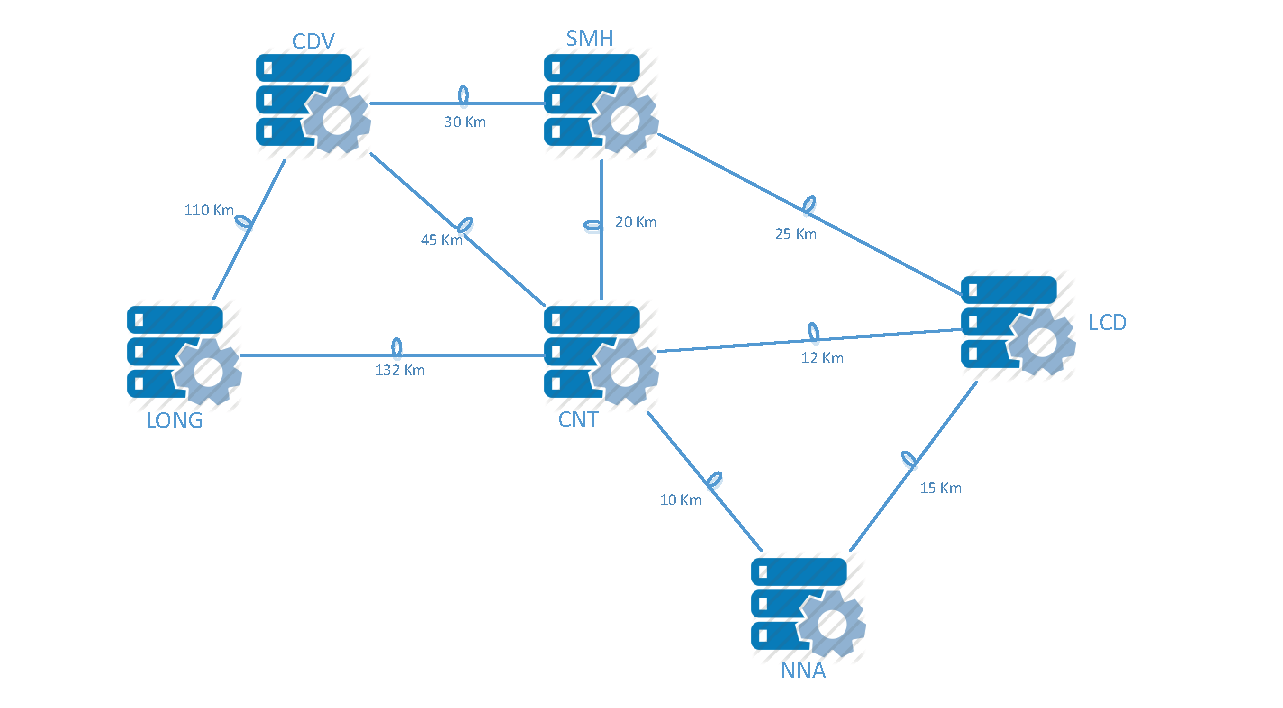
\includegraphics[width=0.8\textwidth]{Imagenes/Diagrama_Fibra_Oscura.eps}
\caption{Diagrama inicial de red oscura preexistente.}
\label{fig:diagrama_red}
\end{figure}

% Para la caracterización y planificación de la red, se consideran 3
% factores claves en todas sus etapas:

% \begin{itemize}
% \item Delay Introducido
% \item Distancia
% \item Costos Monetarios
% \end{itemize}

% Para la Fibra Oscura:

% Si el delay es considerado, se puede incluir cómo un costo adicional
% de distancia (sabiendo la relación entre cantidad de saltos y
% distancia), de tal forma que la minimización ocurra en torno a una
% sola variable.

% Una vez resueltos los costos en una sola variable (Saltos y
% Distancia), se procederá a minimizar la función costo usando el
% conocido algoritmo de Dijkstra.

% Adicionalmente a este procedimiento, para el caso de posibles cortes
% simultáneos, ha de hacerse un estudio probabilístico, dependiendo de
% que tan probable es que se corte una fibra según un umbral ``$\mu$'' se
% dispondrá de una o más rutas alternativas para esta.
